\chapter{Grundlagen}
\section{API}

Der Begriff API steht für \textit{Application Programming Interface} (auf Deutsch: Anwendungs-Programmier-Schnittstelle).
Die Grundlagen heutiger APIs wurden 1952 von David Wheeler, einem Informatikprofessor an der Universität Cambrigde, in einem Leitfaden verfasst.
Dieser Leitfaden beschreibt das Extrahieren einer Bibliothek von Funktionen und Prodzeduren mit einheitlichem, dokumentierten Zugriff \parencite[S.5-6]{wheeler1952use}.
Ira Cotton und Frank Greatorex erwähnten den Begriff erstmalig auf der Fall Joint Computer Konferenz \parencite[S.5]{cotton1968data}.
Dabei erweiterten sie den Leitfaden von David Wheeler um einen wesentlichen Punkt: Der konzeptionellen Trennung der Schnittstelle und Implementierung der Bibliothek.
Somit kann die Implementierung, welche auf die Schnittstelle zugreift, ohne Einfluss auf die Verwender ausgetauscht werden \parencite[S.2]{kress2020graphql}.
APIs sind wie Benutzerschnittstellen, nur ist ein anderer Nutzen dabei im Fokus \parencite[S.5]{berlind2017apis}.
APIs sind also wie Benutzerschnittstellen für die Interaktion mit Benutzern gedacht.
Der wesentliche Unterschied zwischen Benutzerschnittstellen und einer API liegt aber in der Art der Nutzer, die auf das Interface zugreifen.
Bei Benutzerschnittstellen spricht man von einem \textit{human readable interface}, was bedeutet, dass ein menschlicher User mit dem System interagiert.
Bei einer API spricht man von einem \textit{machine readable interface}, also von einer Schnittstelle, die für die Kommunikation zwischen Maschinen gedacht ist.

\section{REST-API}
REST steht für \textit{Representational State Transfer} \parencite[S.235-236]{wheeler1952use}.
REST wurde aufgrund des Erfolgs von SOAP entworfen \parencite[Abs. REST APIs]{graphcms}.
REST ist aber keine konkrete Technologie oder ein Standard.
REST beschreibt einen Architekturstil, welcher im Jahr 2000 von Roy Fielding konzipiert wurde.
Bei REST werden Daten als Ressourcen gesehen und in einem spezifischen Format übertragen.
Ursprünglich wurde von Fielding XML verwendet \parencite[S.11]{kress2020graphql}.
Anders als bei SOAP können REST-APIs aber auch noch andere Datenübertragungsformate wie JSON oder YAML anbieten \parencite[Abs. REST APIs]{graphcms}.
\newline

Zum Vergleich hier ein Buch, welches in JSON und XML repräsentiert wird:
\begin{JsCode}
{
    "isbn": "978-3551555557",
    "title": "Harry Potter und der Orden des Phönix",
    "releaseDate": "2003-11-15T00:00:00.000Z"
}
\end{JsCode}

\begin{XmlCode}
<book>
    <isbn name="isbn" type="string">978-3551555557</isbn>
    <title name="title" type="string">Harry Potter und der Orden des Phönix</title>
    <releaseDate name="isbn" type="dateTime">2003-11-15T00:00:00.000Z</releaseDate>
</book>
\end{XmlCode}

In diesem Beispiel ist ersichtlich, dass JSON (134 Bytes) wesentlich weniger Daten als XML (238 Bytes) beinhaltet.
Zusammenfassend kann man sagen, dass JSON deutlich leichtgewichtiger als XML ist, was sich positiv auf die Datenübertragungszeit auswirkt.

\subsection{REST-Bedingungen}
Als REST-API versteht man eine API welche die REST-Bedingungen erfüllt \parencite[Abs. REST-APIs]{graphcms}.
Die REST-Bedingungen werden wie folgt definiert:

\myparagraph{Einheitliche Schnittstelle}
Der zentrale Unterschied zwischen REST und anderen netzwerkbasiertern Architekturstilen, ist die Definition eines einheitlichen Interfaces \parencite[S.81]{fielding2000architectural}.
Den beteiligten Komponenten wird es ermöglicht sich unabhängig voneinander weiterzuentwickeln.
Um diese unabhängige Weiterentwicklung zu gewährleisten werden Implementierungen von den Services, die sie zur Verfügung stellen, entkoppelt.

\myparagraph{Client-Server-Architektur}
Das Client-Server-Prinzip beschreibt verteilte Systeme.
In diesen verteilten Systemen sendet der Client über eine netzwerkbasierte Verbindung Anfragen an den Server.
In der REST-Architektur sind der Client und der Server klar voneinander abgetrennt.
Damit ist es möglich, beide Komponenten unabhängig voneinander weiterzuentwickeln, ohne dabei Einfluss auf die jeweils andere Kompnente zu haben.

\myparagraph{Zustandslosigkeit}
Zustandlosigkeit bedeutet, dass der Client alle Informationen die der Server benötigt, um eine Anfrage auszuführen, mitsendet.
Diese REST-Bedingung gibt einer REST-API eine Verbesserung der Sichtbarkeit, der Zuverlässigkeit und der Skalierbarkeit \parencite[S. 79]{fielding2000architectural}.

\myparagraph{Schichtenarchitektur}
Geschichtete Systeme sind Systeme, die aus mehreren hierarchischen angeordneten Schichten bestehen.
Dadurch wird eine Architektur geschaffen werden, in der die einzelnen Komponenten nicht über die unmittelbare Schicht, mit der sie interagiert hinaussehen kann.
Mit dieser Architektur wird die Komplexität der Abhängigkeiten innerhalb des Systems reduziert.
Weiters wird die Unabhängigkeit der beteiligten Komponenten gefördert \parencite[S. 79]{fielding2000architectural}.

\myparagraph{Zwischenspeicher}
Um wiederkehrende Anfragen performanter abwickeln zu können, kann dem Server mithilfe des \textit{Cache-Control-Headers} mitgeteilt werden, ob die angefragten Daten zwischengespeichert werden sollen.
Zusätzlich muss definiert werden, wie lange dieser Cache gültig ist.
Nach Ablauf der Gültigkeit werden die Daten erneut vom Server geladen.
Durch das Zwischenspeichern von Daten wird die Performanz des Servers gesteigert.
Ein Nachteil besteht dahingehend, dass dem Client womöglich nicht immer die aktuellsten Daten zur Verfügung stehen \parencite[S. 79]{fielding2000architectural}.

\subsection{Kommunikation mit dem Server}
Die Kommunikation zwischen Server und Client wird bei einer REST-API mittels HTTP und dessen Methoden realisert.
Eine REST-Anfrage besteht aus einem Endpunkt, der HTTP-Methode, den HTTP-Headern und dem HTTP-Body.
Ein Endpunkt enthält eine \textit{URI} welche die Ressource, auf die zugegriffen wird, identifiziert.
\newline

Die HTTP-Methode beschreibt die CRUD-Operation, welche auf die Ressource ausgeführt werden soll.
Um CRUD (Create, Read, Update, Delete) Operationen auf Ressourcen abzusetzen, werden folgende HTTP-Methoden verwendet:
\begin{enumerate}
    \item \textbf{GET: }Wird als lesender Zugriff auf eine Ressource verwendet.
    \item \textbf{POST: }Wird verwendet, um eine neue Ressource zu erstellen.
    \item \textbf{PUT: }Aktualisiert oder ersetzt eine bestehende Ressource.
    \item \textbf{PATCH: }Wird verwendet, um eine Ressource zu bearbeiten.
    \item \textbf{DELETE: }Wird für das Löschen einer Ressource verwendet.
\end{enumerate}

Der HTTP-Header übermittelt bei einer Anfrage zusätzliche Informationen, die für das Caching oder die Authentifizierung benötigt werden.
Der HTTP-Body beinhaltet die Daten, welcher der Client an den Server schicken will.

\subsection{Antwort des Servers auf eine Anfrage}
Da REST-APIs auf dem HTTP-Standard beruhen, wird der zurückgegebene HTTP-Statuscode einer Anfrage verwendet, um den Erfolg oder das Fehlschlagen der Anfrage festzustellen.
Jeder Status-Code gehört zu einer Klasse, jede Klasse wird durch die erste Ziffer des dreistelligen Statuscodes definiert.
Die Statuscodes von 100 bis 199 bedeuten, dass die Antwort eine vorläufige Informationsantwort enthält.
Ein Statuscode Bereich von 200 bis 299 signalisiert eine erfolgreiche Anfrage.
300 bis 399 gibt an den Client die Information zurück, dass die Anfrage an eine andere Ressource weitergeleitet werden muss.
Liegt der zurückgegebene Statuscode zwischen 400 und 499 so hat der Client bei der Anfrage etwas falsch gemacht.
500 bis 599 bedeutet, dass der Fehler am Server passiert ist \parencite[S. 120]{fielding2000architectural}.

\section{GraphQL}
GraphQL wurde 2015 von Facebook für seine eigene Facebook-API veröffentlicht und ist die Spezifikation einer plattformunabhängigen Query-Sprache für APIs \parencite[S. 18]{kress2020graphql}.
GraphQL wurde unter der MIT-Lizenz veröffentlicht.
Die Kommunikation erfolgt wie bei REST über ein Request-Response-Schema.
Für eine Ressource kann es in ERST mehrere Endpunkte geben.
In GraphQL gibt es aber genau einen Endpunkt \parencite[S. 18]{kress2020graphql}.
An diesen Endpunkt werden entweder Querys oder Mutations gesendet.
Querys sind lesende Zugriffe auf Ressourcen, Mutations beschreiben schreibende Zugriffe auf die Ressourcen.
Weiters ermöglicht GraphQL eine bidirektionale Verbindung zwischen Client und Server mittels Subscriptions.
Die Zugriffsmöglichkeiten (Query, Mutation, Subscription) und die von GraphQL verwalteten Objekte werden mittels der \textit{Schema Definition Language SDL} in einem Schema definiert.
In GraphQL werden Ressourcen im Kontext von Graphen gesehen.
Knoten, welche mittels des GraphQL-Schema-Systems definiert werden, repräsentieren Objekte.
Kanten beschreiben die Beziehungen von Objekten im Graphen \parencite[Abs. Basics of a GraphQL API]{rakutenGraphQLVsRest}.
\newline

GraphQL erlaubt es Clients, Daten von mehereren Ressourcen in einer einzigen Abfragequery abzufragen.
Dabei müssen nicht mehr wie bei REST mehrere Abfragen an den Server geschickt werden, um dasselbe Ergebnis zu erzielen.

\begin{figure}[H]
    \centering
    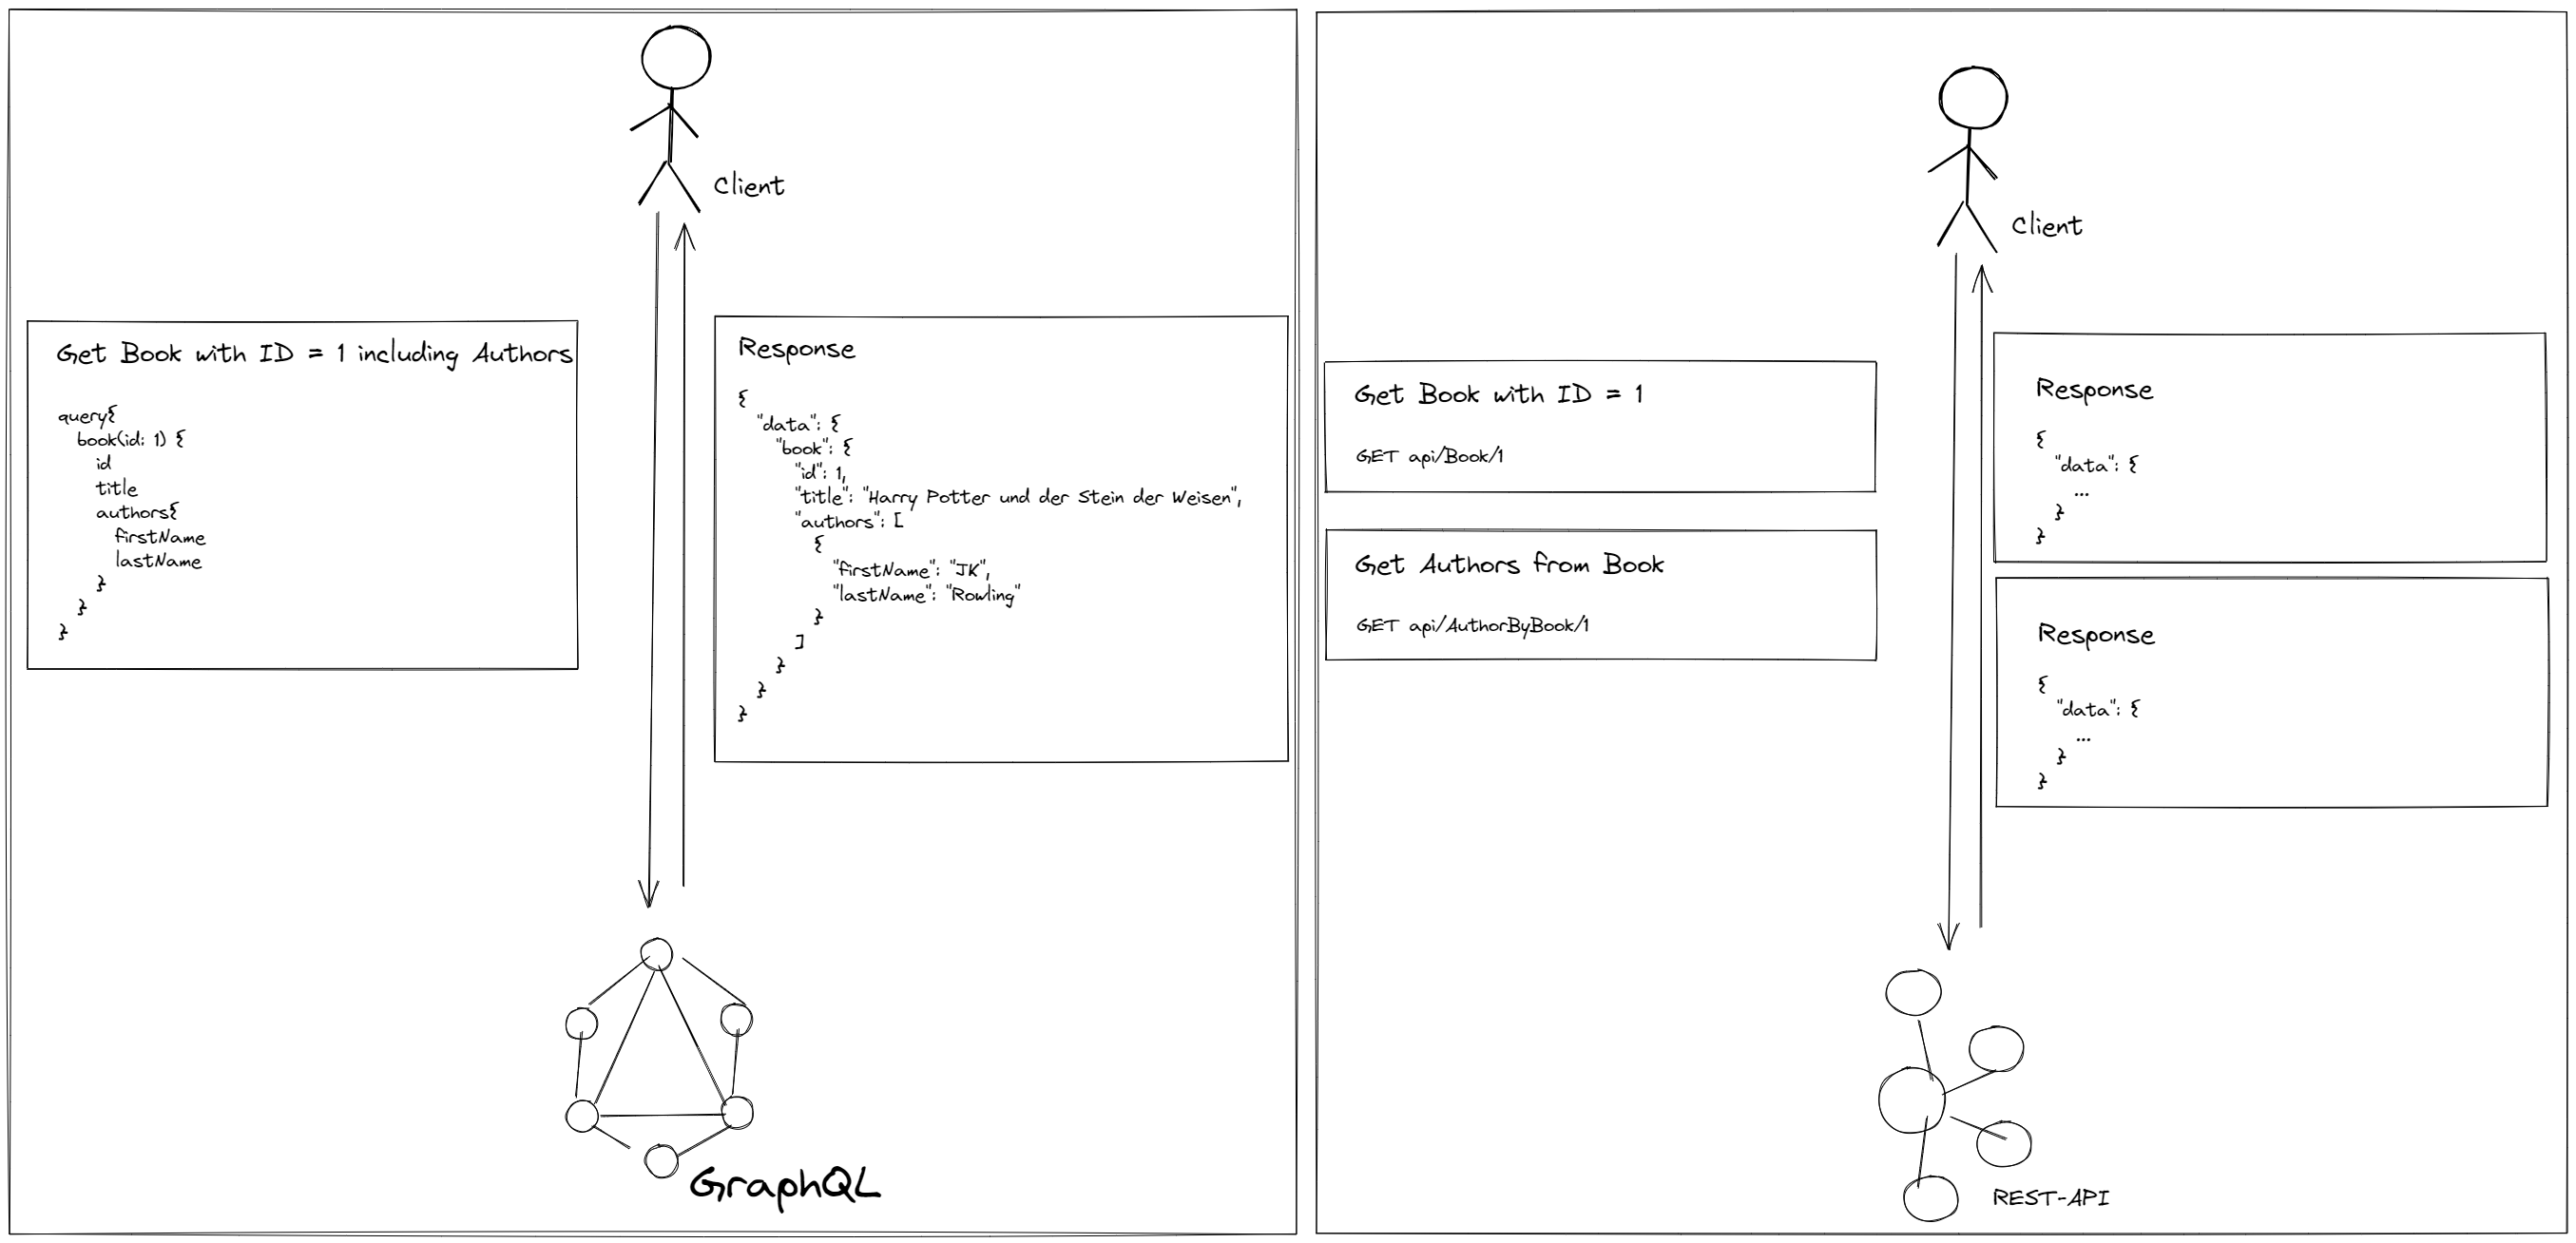
\includegraphics[width=\textwidth]{pics/graphql_rest_request.png}
    \caption{Gegenüberstellung REST-Anfrage / GraphQL-Anfrage}
\end{figure}

In Abbildung 2.1 ist zu sehen, dass ein Client zwei Anfragen an eine REST-API stellen muss, während er bei einem GraphQL-Service nur eine einzige Anfrage benötigt.
Weiters ist zu sehen, dass GraphQL die Daten, welche in der Query abgefragt wurden, genau in der Struktur zurückliefert, in der sie abgefragt wurden.
Dadurch hat GraphQL den Vorteil, dass Antworten auf Anfragen immer vorhersehbar sind \parencite[Abs. Basics of a GraphQL API]{rakutenGraphQLVsRest}.

\subsection{Entwurfsprinzipien}
Da GraphQL sprachunabhängig ist und auch nicht an ein Transportprotokoll gekoppelt ist, werden in der Spezifikation keine Implementierungsdetails definiert, sondern nur Entwurfsprinzipien.
Diese Entwurfsprinzipien werden in den folgenden Abschnitten näher erläutert:

\myparagraph{Produktzentriert}
Die Anforderungen der Clients (Darstellung der Daten) stehen im Mittelpunkt.
GraphQL bietet mit einer Abfragesprache dem Client die Möglichkeit, genau die Daten abzufragen, die er tatsächlich benötigt. Die Hierarchie der
Abfrage wird durch eine Menge ineinander geschachtelter Felder abgebildet \parencite[Abs. 1]{graphqlOnline}.

\myparagraph{Hierarchisch}
Eine GraphQL-Anfrage ist hierarchisch strukturiert.
Jede Anfrage ist so geformt wie die Daten die zurückgelifert werden.
Das bedeutet, dass der Client die Daten genau in dem Format erhält, wie diese in der Anfrage spezifiziert wurden.
Das ist ein intuitiver Weg für den Client, um seine Datenanforderungen zu definieren \parencite[Abs. 1]{graphqlOnline}.

\myparagraph{Strenge Typisierung}
Jeder GraphQL-Service definiert ein anwendungsspezifisches Typsystem.
Anfragen werden im Kontext dieses Typsystems ausgeführt.
Mit Tools wie zum Beispiel \textit{GraphiQL} kann man vor Ausführung der Anfrage sicherstellen, dass sie syntaktisch und semantisch korrekt sind \parencite[Abs. 1]{graphqlOnline}.

\myparagraph{Benutzerdefinierte Antwort}
Mittels des Typsystems definiert der GraphQL-Service ein Schema, welches er veröffentlicht.
In diesem Schema sind die Zugriffsarten als auch die verwalteten Ressourcen definiert.
Der Client ist dafür zuständig, zu definieren, welche Daten er wie abfragen will.
Die meisten anderen Client-Server-Applikationen geben die Form der Daten, welche sie zurückgeben, selbst vor.
Ein GraphQL-Service retourniert exakt die Daten, welche der Client angefordert hat, nicht mehr und nicht weniger \parencite[Abs. 1]{graphqlOnline}.

\myparagraph{Introspektion}
Das Typ-System eines GraphQL-Services kann direkt mit der GraphQL-Abfragesprache abgefragt werden. Diese Abfragen werden für die Erstellung von Tools für GraphQL benötigt \parencite[Abs. 1]{graphqlOnline}.

\section{GraphQL vs. REST}
In den folgenden Abschnitten werden die grundlegenden Unterschiede zwischen REST und GraphQL erläutert.
\subsection{Endpunkte}
Eine REST-API bietet für jede Ressource verschiedene Endpunkte an, um CRUD Operationen für die jeweilige Ressource auszuführen.
GraphQL hingegen bietet nur einen Endpunkt.
An diesen kann der Client eine Abfrage mit einer Query oder einer Mutation senden, um auf die jeweilige Ressource zuzugreifen.

\subsection{Overfetching und Underfetching}
Als Overfetching wird das Laden von zu vielen oder nicht benötigten Daten bezeichnet.
Underfetching bedeutet, dass man mehr Daten benötigt, als der Server dem Client zurückgibt.
Dieses Problem tritt bei REST-APIs auf die viele verschiedene Clients mit Daten versorgen müssen (beispielsweise eine Desktop-Applikation, eine mobile Anwendung und ein Web-Client).
Grundsätzlich wollen alle drei Clients diesselbe Ressourcen abfragen, mit dem Unterschied, dass die mobile Anwendung beispielsweise weniger Daten benötigt.
Die Desktop-Applikation möchte aber alle Daten einer Ressource bekommen, um diese darzustellen.
Eine Lösung dafür wäre beispielsweise, einen Endpunkt für jeden Client zu definieren, um die für ihn benötigen Daten zur Verfügung zu stellen.
Dies resultiert aber in einem erhöten Programmieraufwand und damit auch einer höheren Komplexität der Anwendung.
\newline

Dieses Problem kann bei GraphQL nicht auftreten, da der Client in seiner Anfrage genau jene Daten definiert, die er benötigt.